\section{External packages}
Several packages is used in the code. Here is a brief overview of these.
\subsection{FEniCS}
FEniCS is a package for solving PDEs using the finite element method, and what our code uses to solve the PDE part of the heart equation. FEniCS has a relatively good documentation\cite{FEniCS}, so i will not go into detail here. 

\subsection{gotran}
Gotran is a sympy-based packed for storing stimulation ODEs. ODEs in gotran format are typically stored in \verb .ode  files. From python, you will typically only call the function \verb load_ode(filename) , where filename is the name of the .ode file you want to use. A nice feature of gotran is that is that we can explore the properties of the action potential through the terminal commands \verb gotranprobe  and \verb gotranrun . Gotranprobe is used to check the properties of the ode. A typical run may look something like this

\begin{verbatim}
/simula_summer13$ gotranprobe myocyte.ode 
Loaded ODE model 'myocyte' with:
            Num states: 30
      Num field states: 1
        Num parameters: 2
  Num field parameters: 2
         Num variables: 2
Information of myocyte Gotran model
States: Ca_c, Ca_d, Ca_i, Ca_rel, Ca_up, F1, F2, K_c, K_i, Na_c, Na_i, O, O_C,
O_Calse, O_TC, O_TMgC, O_TMgMg, V, a_ur, d_L, f_L1, f_L2, h1, h2, i_ur, m, n, 
pa, r, s
Parameters: g_K1, ist
\end{verbatim}
which gives us information on the ode. This is a coupled system of 30 ODEs, with 2 parameters. The names of the states and parameters are usually very cryptic, as in this case. However, the potential difference is usally called V (sometimes a lowercase v). To all parameters are given default values, but they can be set as well. In order to check the action potential, we can use the \verb gotranrun  function. 

This will look something like this
\begin{verbatim}
 /simula_summer13$ gotranrun myocyte.ode --plot_states V --code.language C 
 --parameters ist -10 --tstop 300
\end{verbatim}
which will produce a plot like the one shown in Fig. \ref{fig:gotran}. The \verb plot_states  keyword selects what state to plot (typically we want this to be V or v), the parameter keyword sets the parameters. From the myocyte model, we need to apply some stimulation for the activation to take place. This varies from model to model. The tstop keyword select how long to solve for, and lastly, the code.language is set to C for improved speed. 
% 
\begin{figure}
 \centering
 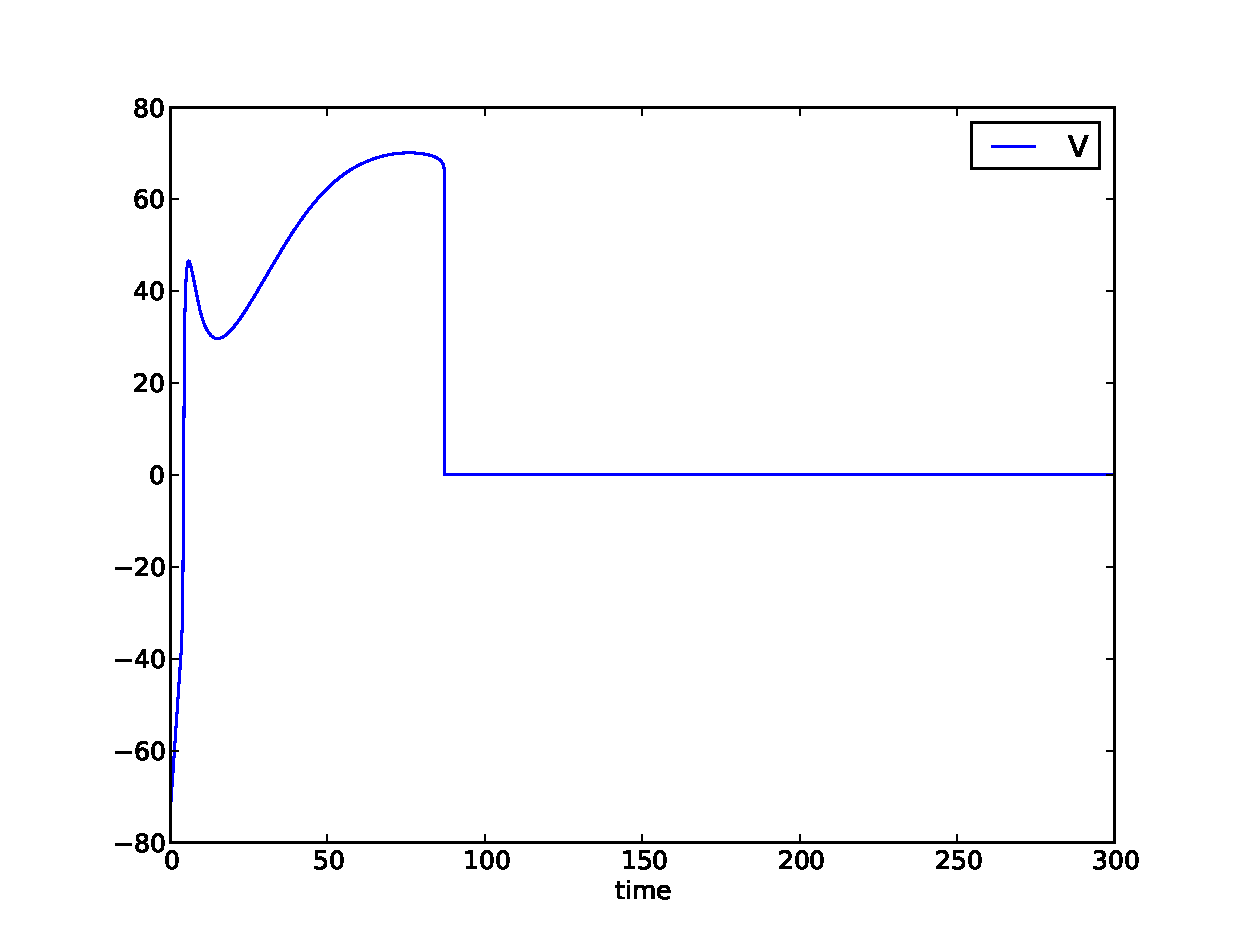
\includegraphics[width=10cm]{figures/gotran.eps}
 \caption{\label{fig:gotran} A possible activation potential.}
\end{figure}


\subsection{goss}
Goss is the package used to solve the ODEs stored by gotran. we initialize an ode by writing 
\begin{lstlisting}
	from dolfin import *
	from goss import *
	from gotran import load_ode

	#Fenics part
	mesh = UnitSquareMesh(10, 10) 
	space = FunctionSpace(mesh, 'Lagrange', 1)
	vertex_to_dof_map =  space.dofmap().vertex_to_dof_map(mesh)
	
	### Setting up Goss/Gotran part
	ode = jit(load_ode("myocyte.ode"))
	N_thread = mesh.coordinates().shape[0]
	fenics_ordered_coordinates = mesh.coordinates()[vertex_to_dof_map]
	P0 = make_parameter_field(fenics_ordered_coordinates, ode)
	solver = ImplicitEuler()
	ode_solver = ODESystemSolver(int(N_thread), solver, ode)
\end{lstlisting}
Let's go through the goss/gotran part line by line. The first line loads the ode ``myocyte.ode''. The second line sets the number of states to solve for (goss actually solve these side by side). The third line produces an array with coordinates that is ordered in the same way as the solution vector produced by FEniCS and stores this to \verb fenics_ordered_coordinates . The fourth line sets the parameters as illustrated in the previous section. Note that this is not a goss function, but a self-defined one. The fifth line sets the time solver method, and finally the last line creates the solver. The solver can then advance by \verb ode_solver.advance(dt,time) , and the states can be set or get by \verb ode_solver.set_field_states(new_states)  and \\ \verb ode_solver.get_field_states(state_vector) . Note that \verb state_vector must by preallocated, and will be filled with the solver states for the potential difference. 

\subsubsection{time solvers}
goss has a variety of different time solvers. Here are some of them 
\begin{itemize}
 \item \verb ExplicitEuler()  - first order explicit euler. Very unstable, do not use.
 
 \item \verb ImplicitEuler()  - first order implicit euler. This one is very stable and good for testing
 
 \item \verb ThetaSolver()  - Theta rule. Has a parameter theta, that is initially set to 0.5, which gives a semi-implicit 2nd order scheme. Theta can also be manipulated directly. 1 gives Forward Euler, 0 gives backward Euler. 
 
 \item \verb GRL2()  - 2nd order explicit method. This is quite stable. A (norwegian) description of the method can be found in \cite{Else10} p. 53-54.
\end{itemize}



